% GNUPLOT: LaTeX picture with Postscript
\begingroup
  \makeatletter
  \providecommand\color[2][]{%
    \GenericError{(gnuplot) \space\space\space\@spaces}{%
      Package color not loaded in conjunction with
      terminal option `colourtext'%
    }{See the gnuplot documentation for explanation.%
    }{Either use 'blacktext' in gnuplot or load the package
      color.sty in LaTeX.}%
    \renewcommand\color[2][]{}%
  }%
  \providecommand\includegraphics[2][]{%
    \GenericError{(gnuplot) \space\space\space\@spaces}{%
      Package graphicx or graphics not loaded%
    }{See the gnuplot documentation for explanation.%
    }{The gnuplot epslatex terminal needs graphicx.sty or graphics.sty.}%
    \renewcommand\includegraphics[2][]{}%
  }%
  \providecommand\rotatebox[2]{#2}%
  \@ifundefined{ifGPcolor}{%
    \newif\ifGPcolor
    \GPcolortrue
  }{}%
  \@ifundefined{ifGPblacktext}{%
    \newif\ifGPblacktext
    \GPblacktexttrue
  }{}%
  % define a \g@addto@macro without @ in the name:
  \let\gplgaddtomacro\g@addto@macro
  % define empty templates for all commands taking text:
  \gdef\gplbacktext{}%
  \gdef\gplfronttext{}%
  \makeatother
  \ifGPblacktext
    % no textcolor at all
    \def\colorrgb#1{}%
    \def\colorgray#1{}%
  \else
    % gray or color?
    \ifGPcolor
      \def\colorrgb#1{\color[rgb]{#1}}%
      \def\colorgray#1{\color[gray]{#1}}%
      \expandafter\def\csname LTw\endcsname{\color{white}}%
      \expandafter\def\csname LTb\endcsname{\color{black}}%
      \expandafter\def\csname LTa\endcsname{\color{black}}%
      \expandafter\def\csname LT0\endcsname{\color[rgb]{1,0,0}}%
      \expandafter\def\csname LT1\endcsname{\color[rgb]{0,1,0}}%
      \expandafter\def\csname LT2\endcsname{\color[rgb]{0,0,1}}%
      \expandafter\def\csname LT3\endcsname{\color[rgb]{1,0,1}}%
      \expandafter\def\csname LT4\endcsname{\color[rgb]{0,1,1}}%
      \expandafter\def\csname LT5\endcsname{\color[rgb]{1,1,0}}%
      \expandafter\def\csname LT6\endcsname{\color[rgb]{0,0,0}}%
      \expandafter\def\csname LT7\endcsname{\color[rgb]{1,0.3,0}}%
      \expandafter\def\csname LT8\endcsname{\color[rgb]{0.5,0.5,0.5}}%
    \else
      % gray
      \def\colorrgb#1{\color{black}}%
      \def\colorgray#1{\color[gray]{#1}}%
      \expandafter\def\csname LTw\endcsname{\color{white}}%
      \expandafter\def\csname LTb\endcsname{\color{black}}%
      \expandafter\def\csname LTa\endcsname{\color{black}}%
      \expandafter\def\csname LT0\endcsname{\color{black}}%
      \expandafter\def\csname LT1\endcsname{\color{black}}%
      \expandafter\def\csname LT2\endcsname{\color{black}}%
      \expandafter\def\csname LT3\endcsname{\color{black}}%
      \expandafter\def\csname LT4\endcsname{\color{black}}%
      \expandafter\def\csname LT5\endcsname{\color{black}}%
      \expandafter\def\csname LT6\endcsname{\color{black}}%
      \expandafter\def\csname LT7\endcsname{\color{black}}%
      \expandafter\def\csname LT8\endcsname{\color{black}}%
    \fi
  \fi
    \setlength{\unitlength}{0.0500bp}%
    \ifx\gptboxheight\undefined%
      \newlength{\gptboxheight}%
      \newlength{\gptboxwidth}%
      \newsavebox{\gptboxtext}%
    \fi%
    \setlength{\fboxrule}{0.5pt}%
    \setlength{\fboxsep}{1pt}%
    \definecolor{tbcol}{rgb}{1,1,1}%
\begin{picture}(11520.00,14400.00)%
    \gplgaddtomacro\gplbacktext{%
      \csname LTb\endcsname%%
      \put(793,9950){\makebox(0,0)[r]{\strut{}1.0}}%
      \csname LTb\endcsname%%
      \put(793,10317){\makebox(0,0)[r]{\strut{}1.4}}%
      \csname LTb\endcsname%%
      \put(793,10707){\makebox(0,0)[r]{\strut{}2.0}}%
      \csname LTb\endcsname%%
      \put(793,11074){\makebox(0,0)[r]{\strut{}2.8}}%
      \csname LTb\endcsname%%
      \put(793,11463){\makebox(0,0)[r]{\strut{}4.0}}%
      \csname LTb\endcsname%%
      \put(793,11830){\makebox(0,0)[r]{\strut{}5.6}}%
      \csname LTb\endcsname%%
      \put(793,12219){\makebox(0,0)[r]{\strut{}8.0}}%
      \csname LTb\endcsname%%
      \put(793,12566){\makebox(0,0)[r]{\strut{}11.0}}%
      \csname LTb\endcsname%%
      \put(793,12933){\makebox(0,0)[r]{\strut{}15.4}}%
      \csname LTb\endcsname%%
      \put(793,13322){\makebox(0,0)[r]{\strut{}22.0}}%
    }%
    \gplgaddtomacro\gplfronttext{%
      \csname LTb\endcsname%%
      \put(195,11748){\rotatebox{-270}{\makebox(0,0){\strut{}(a) Relative execution time}}}%
      \csname LTb\endcsname%%
      \put(3485,14164){\makebox(0,0)[r]{\strut{}\VericertBase}}%
      \csname LTb\endcsname%%
      \put(3485,13924){\makebox(0,0)[r]{\strut{}\VericertList}}%
      \csname LTb\endcsname%%
      \put(7206,14164){\makebox(0,0)[r]{\strut{}\VericertHyper}}%
      \csname LTb\endcsname%%
      \put(7206,13924){\makebox(0,0)[r]{\strut{}\BambuNoOpt}}%
      \csname LTb\endcsname%%
      \put(10927,14164){\makebox(0,0)[r]{\strut{}\BambuDefault}}%
    }%
    \gplgaddtomacro\gplbacktext{%
      \csname LTb\endcsname%%
      \put(793,7951){\makebox(0,0)[r]{\strut{}1.0}}%
      \csname LTb\endcsname%%
      \put(793,8198){\makebox(0,0)[r]{\strut{}1.6}}%
      \csname LTb\endcsname%%
      \put(793,8446){\makebox(0,0)[r]{\strut{}2.5}}%
      \csname LTb\endcsname%%
      \put(793,8693){\makebox(0,0)[r]{\strut{}4.0}}%
      \csname LTb\endcsname%%
      \put(793,8940){\makebox(0,0)[r]{\strut{}6.3}}%
      \csname LTb\endcsname%%
      \put(793,9188){\makebox(0,0)[r]{\strut{}10.0}}%
      \csname LTb\endcsname%%
      \put(793,9435){\makebox(0,0)[r]{\strut{}15.8}}%
      \csname LTb\endcsname%%
      \put(793,9682){\makebox(0,0)[r]{\strut{}25.0}}%
    }%
    \gplgaddtomacro\gplfronttext{%
      \csname LTb\endcsname%%
      \put(195,8788){\rotatebox{-270}{\makebox(0,0){\strut{}(b) Rel. cycle count}}}%
    }%
    \gplgaddtomacro\gplbacktext{%
      \csname LTb\endcsname%%
      \put(793,5953){\makebox(0,0)[r]{\strut{}0.0}}%
      \csname LTb\endcsname%%
      \put(793,6278){\makebox(0,0)[r]{\strut{}2.0}}%
      \csname LTb\endcsname%%
      \put(793,6603){\makebox(0,0)[r]{\strut{}4.0}}%
      \csname LTb\endcsname%%
      \put(793,6928){\makebox(0,0)[r]{\strut{}6.0}}%
      \csname LTb\endcsname%%
      \put(793,7253){\makebox(0,0)[r]{\strut{}8.0}}%
      \csname LTb\endcsname%%
      \put(793,7578){\makebox(0,0)[r]{\strut{}10.0}}%
    }%
    \gplgaddtomacro\gplfronttext{%
      \csname LTb\endcsname%%
      \put(195,6847){\rotatebox{-270}{\makebox(0,0){\strut{}(c) Delay (ns)}}}%
    }%
    \gplgaddtomacro\gplbacktext{%
      \csname LTb\endcsname%%
      \put(793,1750){\makebox(0,0)[r]{\strut{}0.70}}%
      \csname LTb\endcsname%%
      \put(793,2146){\makebox(0,0)[r]{\strut{}0.83}}%
      \csname LTb\endcsname%%
      \put(793,2578){\makebox(0,0)[r]{\strut{}1.00}}%
      \csname LTb\endcsname%%
      \put(793,3002){\makebox(0,0)[r]{\strut{}1.20}}%
      \csname LTb\endcsname%%
      \put(793,3426){\makebox(0,0)[r]{\strut{}1.44}}%
      \csname LTb\endcsname%%
      \put(793,3849){\makebox(0,0)[r]{\strut{}1.73}}%
      \csname LTb\endcsname%%
      \put(793,4273){\makebox(0,0)[r]{\strut{}2.07}}%
      \csname LTb\endcsname%%
      \put(793,4697){\makebox(0,0)[r]{\strut{}2.49}}%
      \csname LTb\endcsname%%
      \put(793,5131){\makebox(0,0)[r]{\strut{}3.00}}%
      \csname LTb\endcsname%%
      \put(793,5544){\makebox(0,0)[r]{\strut{}3.58}}%
      \csname LTb\endcsname%%
      \put(1078,1649){\rotatebox{-90}{\makebox(0,0)[l]{\strut{}\y{2mm}}}}%
      \csname LTb\endcsname%%
      \put(1446,1649){\rotatebox{-90}{\makebox(0,0)[l]{\strut{}\y{3mm}}}}%
      \csname LTb\endcsname%%
      \put(1814,1649){\rotatebox{-90}{\makebox(0,0)[l]{\strut{}\y{adi}}}}%
      \csname LTb\endcsname%%
      \put(2182,1649){\rotatebox{-90}{\makebox(0,0)[l]{\strut{}\y{atas}}}}%
      \csname LTb\endcsname%%
      \put(2550,1649){\rotatebox{-90}{\makebox(0,0)[l]{\strut{}\y{bicg}}}}%
      \csname LTb\endcsname%%
      \put(2918,1649){\rotatebox{-90}{\makebox(0,0)[l]{\strut{}\y{cholesky}}}}%
      \csname LTb\endcsname%%
      \put(3286,1649){\rotatebox{-90}{\makebox(0,0)[l]{\strut{}\y{covariance}}}}%
      \csname LTb\endcsname%%
      \put(3654,1649){\rotatebox{-90}{\makebox(0,0)[l]{\strut{}\y{doitgen}}}}%
      \csname LTb\endcsname%%
      \put(4022,1649){\rotatebox{-90}{\makebox(0,0)[l]{\strut{}\y{durbin}}}}%
      \csname LTb\endcsname%%
      \put(4390,1649){\rotatebox{-90}{\makebox(0,0)[l]{\strut{}\y{fdtd-2d}}}}%
      \csname LTb\endcsname%%
      \put(4758,1649){\rotatebox{-90}{\makebox(0,0)[l]{\strut{}\y{floyd-warshall}}}}%
      \csname LTb\endcsname%%
      \put(5126,1649){\rotatebox{-90}{\makebox(0,0)[l]{\strut{}\y{gemm}}}}%
      \csname LTb\endcsname%%
      \put(5494,1649){\rotatebox{-90}{\makebox(0,0)[l]{\strut{}\y{gemver}}}}%
      \csname LTb\endcsname%%
      \put(5862,1649){\rotatebox{-90}{\makebox(0,0)[l]{\strut{}\y{gesummv}}}}%
      \csname LTb\endcsname%%
      \put(6230,1649){\rotatebox{-90}{\makebox(0,0)[l]{\strut{}\y{heat-3d}}}}%
      \csname LTb\endcsname%%
      \put(6598,1649){\rotatebox{-90}{\makebox(0,0)[l]{\strut{}\y{jacobi-1d}}}}%
      \csname LTb\endcsname%%
      \put(6966,1649){\rotatebox{-90}{\makebox(0,0)[l]{\strut{}\y{jacobi-2d}}}}%
      \csname LTb\endcsname%%
      \put(7334,1649){\rotatebox{-90}{\makebox(0,0)[l]{\strut{}\y{lu}}}}%
      \csname LTb\endcsname%%
      \put(7701,1649){\rotatebox{-90}{\makebox(0,0)[l]{\strut{}\y{ludcmp}}}}%
      \csname LTb\endcsname%%
      \put(8069,1649){\rotatebox{-90}{\makebox(0,0)[l]{\strut{}\y{mvt}}}}%
      \csname LTb\endcsname%%
      \put(8437,1649){\rotatebox{-90}{\makebox(0,0)[l]{\strut{}\y{nussinov}}}}%
      \csname LTb\endcsname%%
      \put(8805,1649){\rotatebox{-90}{\makebox(0,0)[l]{\strut{}\y{seidel-2d}}}}%
      \csname LTb\endcsname%%
      \put(9173,1649){\rotatebox{-90}{\makebox(0,0)[l]{\strut{}\y{symm}}}}%
      \csname LTb\endcsname%%
      \put(9541,1649){\rotatebox{-90}{\makebox(0,0)[l]{\strut{}\y{syr2k}}}}%
      \csname LTb\endcsname%%
      \put(9909,1649){\rotatebox{-90}{\makebox(0,0)[l]{\strut{}\y{syrk}}}}%
      \csname LTb\endcsname%%
      \put(10277,1649){\rotatebox{-90}{\makebox(0,0)[l]{\strut{}\y{trisolv}}}}%
      \csname LTb\endcsname%%
      \put(10645,1649){\rotatebox{-90}{\makebox(0,0)[l]{\strut{}\y{trmm}}}}%
      \csname LTb\endcsname%%
      \put(11013,1649){\rotatebox{-90}{\makebox(0,0)[l]{\strut{}\y{median}}}}%
    }%
    \gplgaddtomacro\gplfronttext{%
      \csname LTb\endcsname%%
      \put(195,3775){\rotatebox{-270}{\makebox(0,0){\strut{}(d) Relative area}}}%
    }%
    \gplbacktext
    \put(0,0){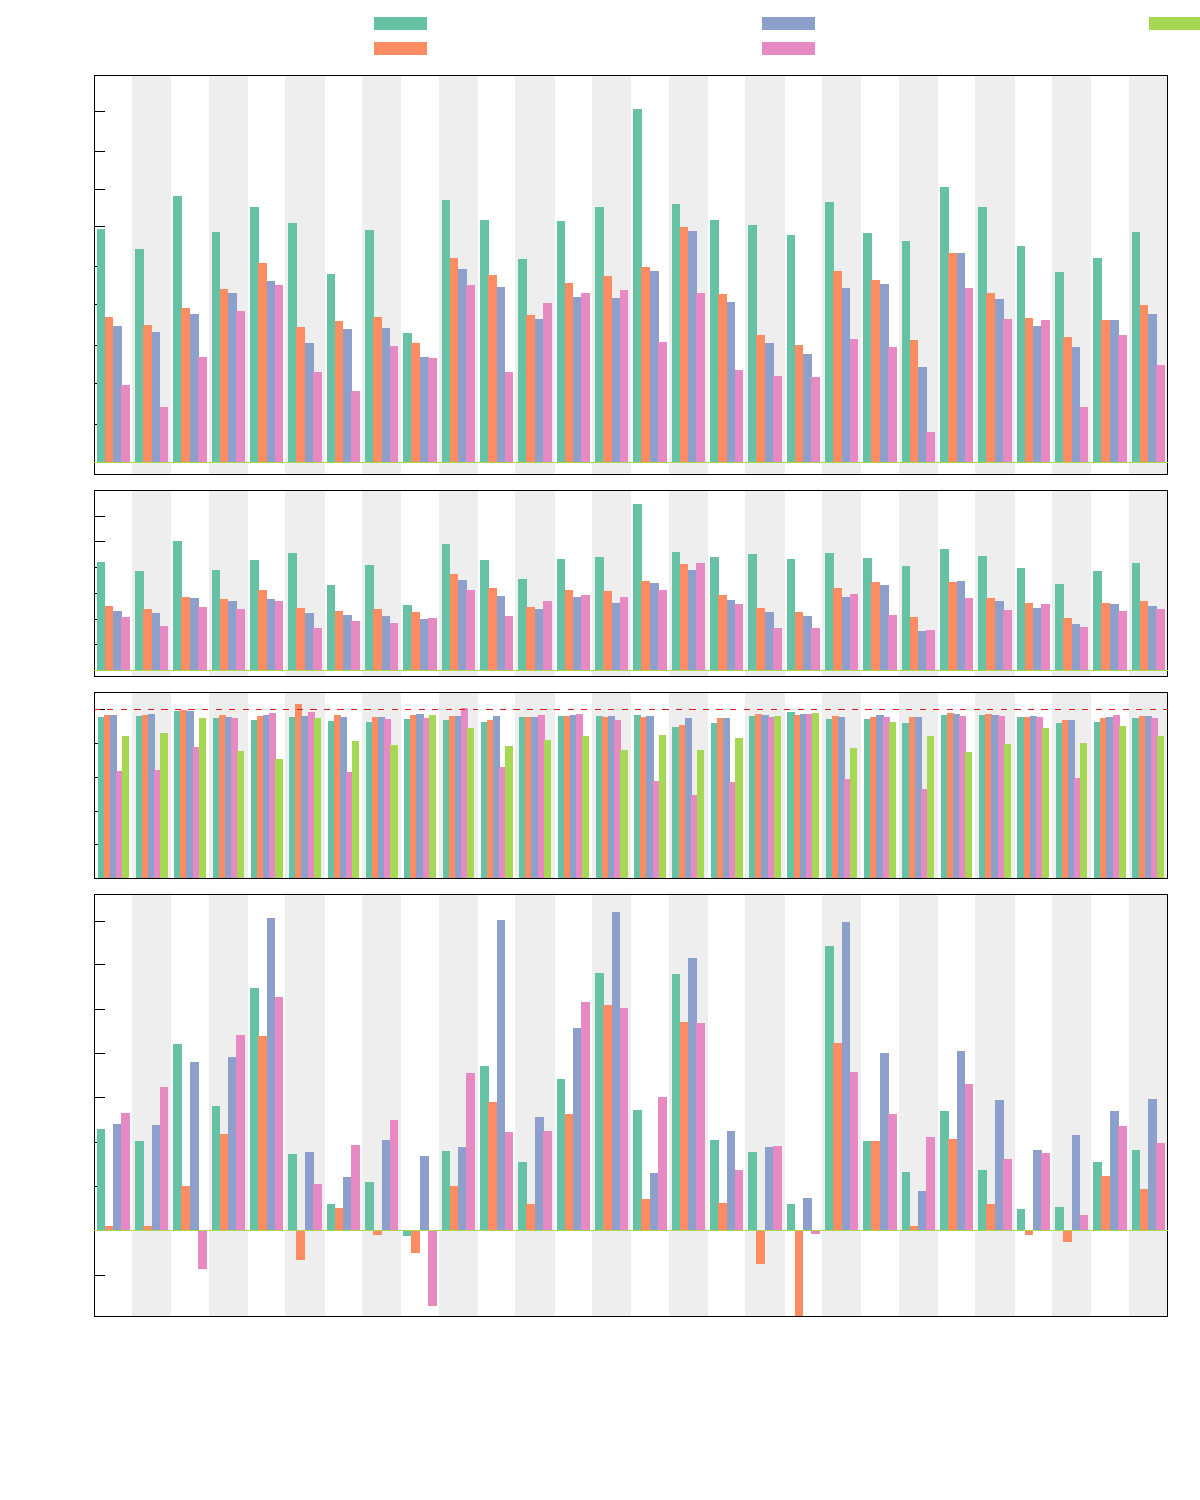
\includegraphics[width={576.00bp},height={720.00bp}]{bar-plot-full}}%
    \gplfronttext
  \end{picture}%
\endgroup
